
%%%%%%%%%%%%%
%     FUTURE WORK    %
%%%%%%%%%%%%%

\begin{figure}
\centering
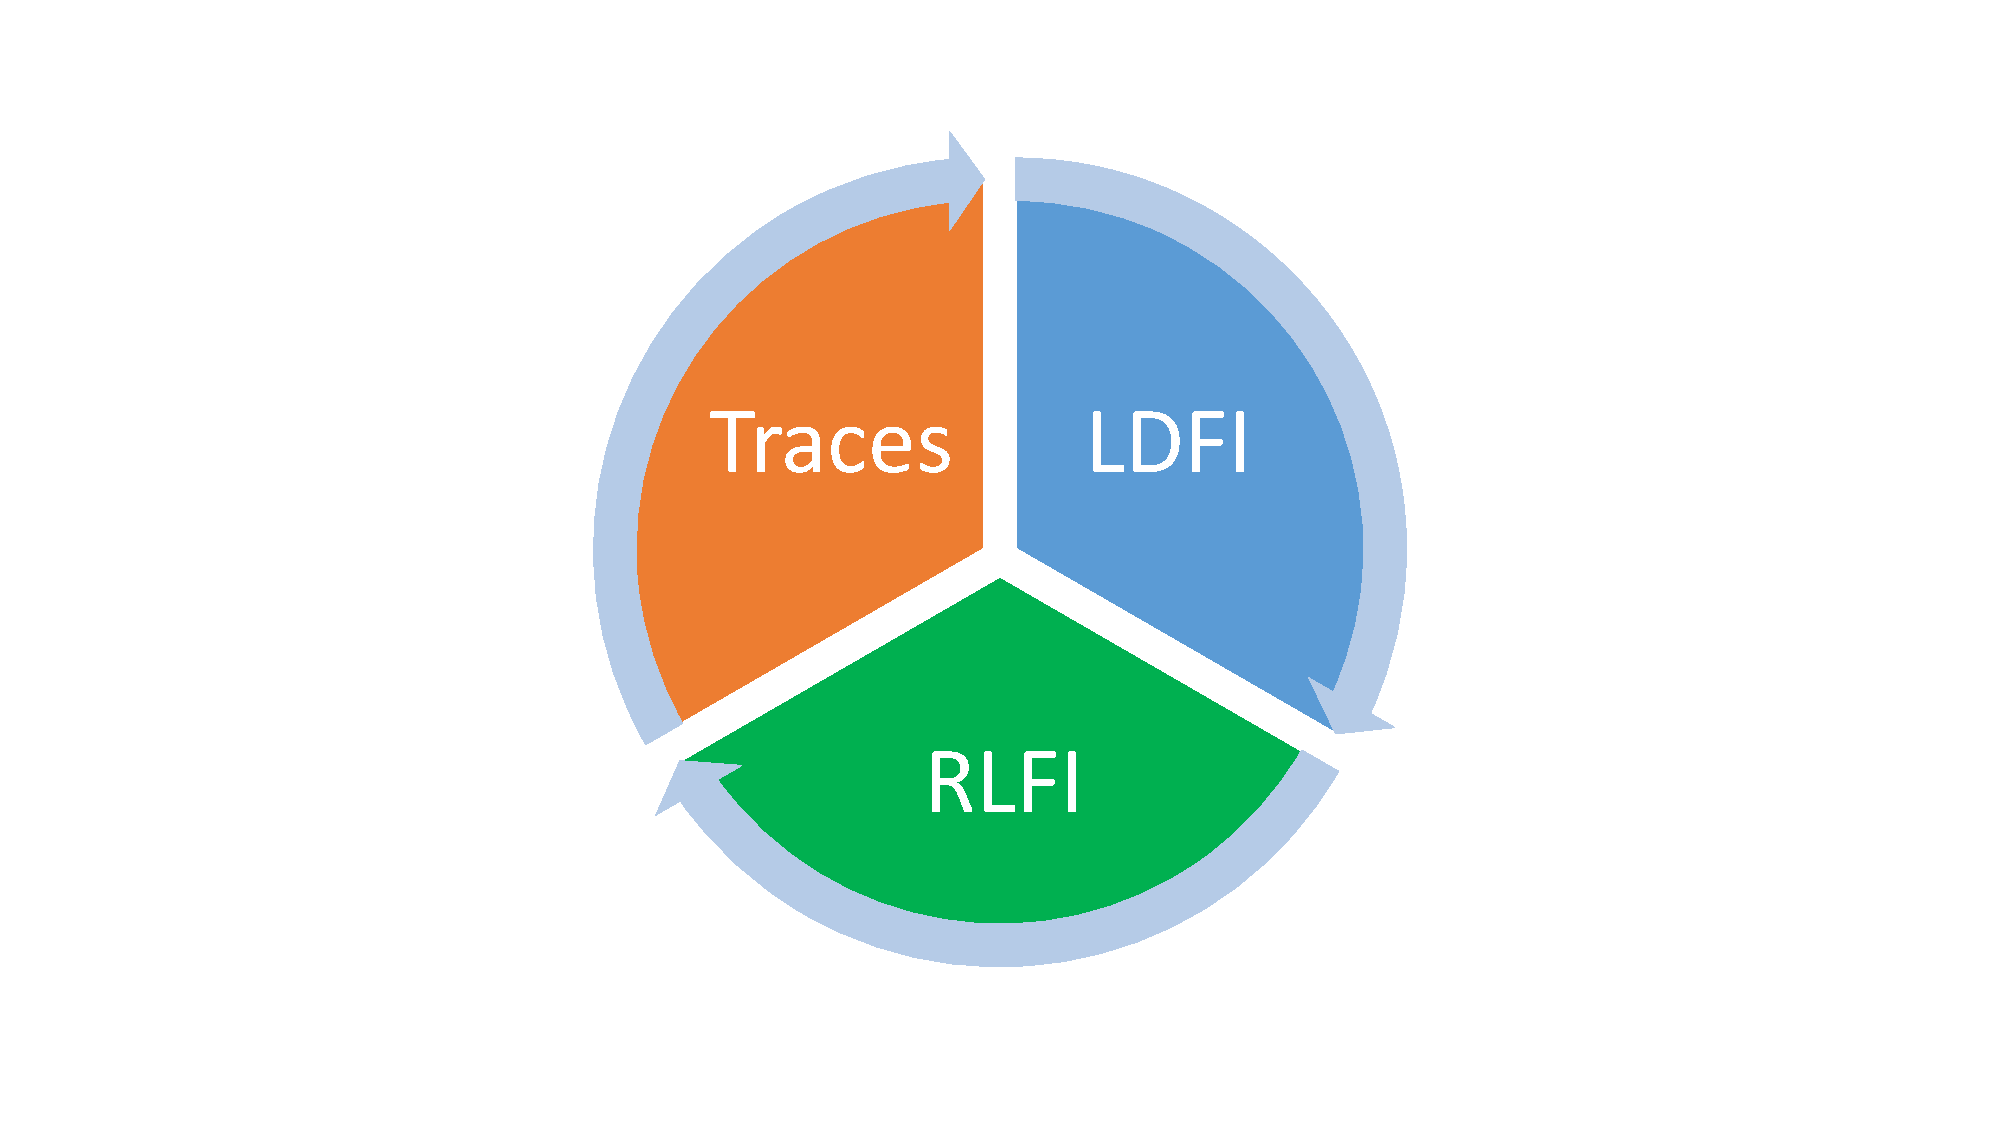
\includegraphics[width=8cm,height=10cm,keepaspectratio=true]{puzzle}
\caption{Fine-grained tracing, LDFI and RLFI completing the puzzle of debugging distributed systems}
\label{puzzle}
\end{figure}

\section{Future Work}
\kmd{need more future directions.}
The current implementation of RLFI is a proof-of-concept to show the utility and efficiency of the approach to fault injection experiments. Our current focus is extending the implementation to support a multitude of languages, not just Golang. 

It is next to impossible to obtain a real life service from industry partners to perform our tests on, mainly because our partners do not want to risk compromising service integrity or jeopardizing confidential information such as software architecture and client data. Also, when compared to the real world, the toy architectures examined in the evaluation are practically trivial. 

Manually digging through traces to find interesting points of failure for RLFI is a daunting task to say the least. PyLDFI, an implementation of Lineage Driven Fault Injection, is pioneered by researchers at UC Santa Cruz \kmd{need technical report on pyLDFI to cite here} capable of pinpointing failure scenarios ideal for FI experiments driven by RLFI. We can feed the good traces produced by the underlying into LDFI, which will find identify critical points of failure. With the critical points found, we carefully inject the faults into the system and determine whether the fault handling mechanism of the service is sufficient. We continue such a cycle of tracing, reasoning, and injecting failures until we identify enough devastating bugs to preoccupy the lives of project systems builders or, in the absence of bugs, are thoroughly convinced of the correctness of the implementation.

Currently the traces resulting from our framework are cluttered and require parsing to support legibility. We would like to develop a small, offline tool capable of transforming the traces into something PyLDFI can understand and also produce a visual call graph for ease of verification. 

%%%%%%%
%    EOF     %
%%%%%%%